% Asset ID: A21DifferentiationTikZ-003
% Source: Chapter 9 implicit differentiation evidence
% Related lesson section: Implicit differentiation
% Purpose: Show dy/dx = -x/y for x^2 + y^2 = 16 via tangent-radius perpendicularity.
\documentclass[tikz,border=8pt]{standalone}
\usepackage{amsmath}
\usetikzlibrary{calc}
\begin{document}
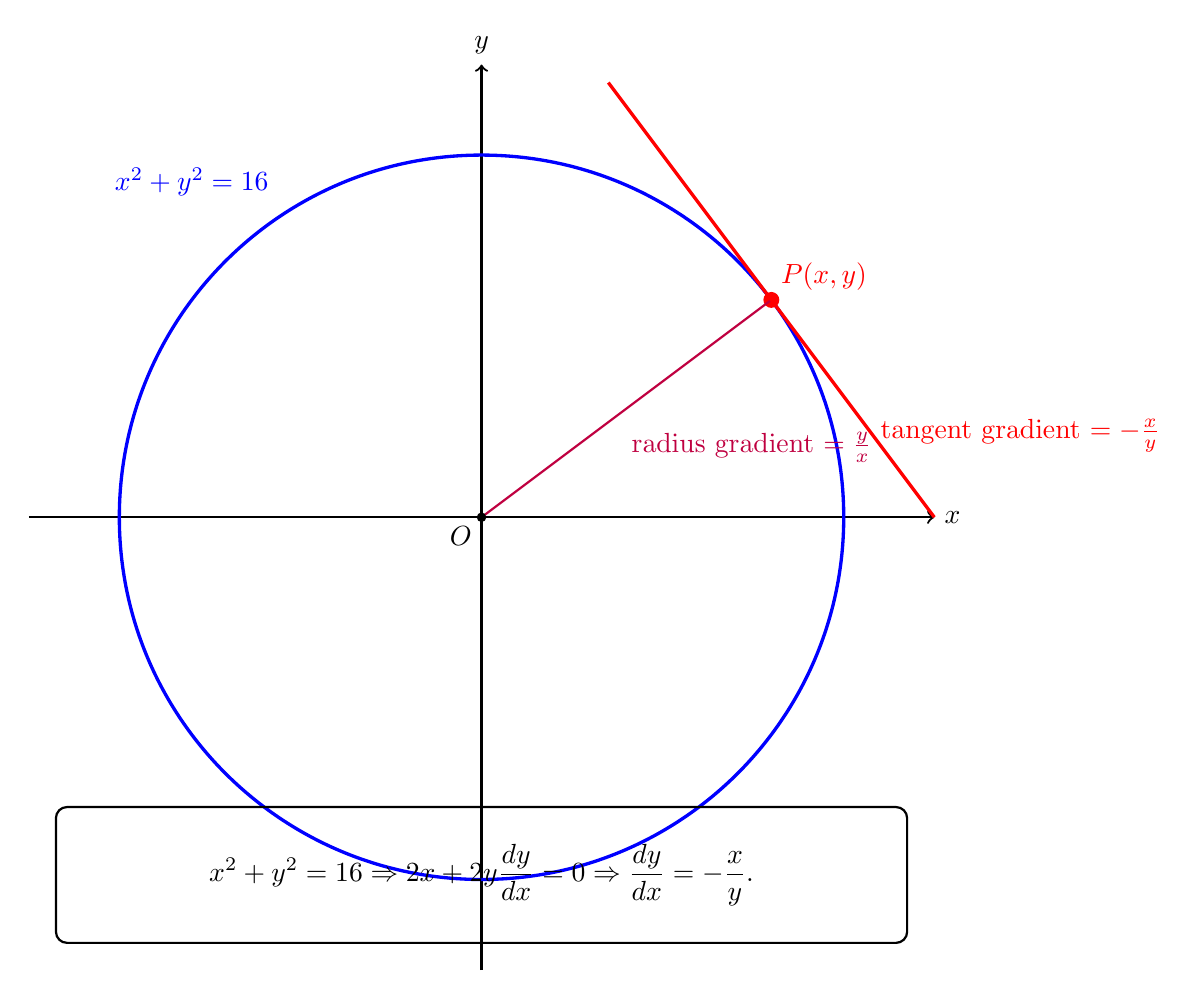
\begin{tikzpicture}[scale=1.15]
\draw[->, thick] (-5,0) -- (5,0) node[right] {$x$};
\draw[->, thick] (0,-5) -- (0,5) node[above] {$y$};
\draw[very thick, blue] (0,0) circle (4);
\node[blue] at (-3.2,3.7) {$x^2+y^2=16$};
\coordinate (P) at (3.2,2.4);
\fill[red] (P) circle (2.5pt);
\node[above right, red] at (P) {$P(x,y)$};
\draw[thick, purple] (0,0) -- (P);
\node[purple, below right] at (1.55,1.05) {radius gradient \(=\frac{y}{x}\)};
\draw[very thick, red] ($(P)+(-1.8,2.4)$) -- ($(P)+(1.8,-2.4)$);
\node[red, right] at ($(P)+(1.1,-1.5)$) {tangent gradient \(=-\frac{x}{y}\)};
\fill[black] (0,0) circle (1.5pt);
\node[below left] at (0,0) {$O$};
\draw[rounded corners, thick] (-4.7,-4.7) rectangle (4.7,-3.2);
\node[align=center] at (0,-3.95) {\(\displaystyle x^2+y^2=16\Rightarrow 2x+2y\frac{dy}{dx}=0\Rightarrow \frac{dy}{dx}=-\frac{x}{y}\).};
\end{tikzpicture}
\end{document}
